\section{Formulas and Basic Math}

\subsection{Roots}

\begin{align*}
    \sqrt[n]{a}\cdot\sqrt[n]{b} & = \sqrt[n]{a\cdot b} \\
    \frac{\sqrt[n]{a}}{\sqrt[n]{b}} & = \sqrt[n]{\frac{a}{b}} \\
    (\sqrt[n]{a})^m & = \sqrt[n]{a^m} \\
    \sqrt[m]{\sqrt[n]{a}} & = \sqrt[m\cdot n]{a}
\end{align*}

\subsection{Logarithm}

\begin{align*}
    \log_n(a\cdot b) & = \log_n(a) + \log_n(b) \\
    \log_n(a\div b) & = \log_n(a) - \log_n(b) \\
    \log_n(a^b) & = b \cdot \log_n(a)
\end{align*}

\subsection{Quadratic Fromula}
\begin{align*}
    x = \frac{-b\pm\sqrt{b^2 - 4ac}}{2a}
\end{align*}

With discriminant $b^2-4ac$:
\begin{enumerate}
    \item $b^2-4ac > 0$, there are \em{two distinct real solutions}
    \item $b^2-4ac = 0$, there is \em{one real solution}
    \item $b^2-4ac < 0$, there are \em{no real solutions}
\end{enumerate}

\subsection{Trigonometry}

\textbf{``Normal''}
\begin{align*}
    \tan\theta & = \frac{\sin\theta}{\cos\theta} \\
    1\div\cot(x) & = \tan(x) \\
    \sin -\theta & = -\sin\theta\text{ (cos and tan same)} \\
    \sin 2\theta & = 2\sin\theta\cos\theta \\
    \cos 2\theta & = 2\cos^2\theta - \sin^2\theta = 2\cos^2\theta - 1 = 1 - 2\sin^2\theta \\
    \sin(\alpha \pm \beta) & = \sin\alpha\cos\beta\pm\cos\alpha\sin\beta \\
    \cos(\alpha\pm\beta) & = \cos\alpha\cos\beta \mp \sin\alpha\sin\beta \\
\end{align*}
\textbf{Hyperbolic}
\begin{align*}
    \sinh x & = \frac{e^x - e^{-x}}{2}=\frac{e^{2x}-1}{2e^x} \\
    \cosh x & = \frac{e^x + e^{-x}}{2} = \frac{e^{2x}+1}{2e^x} \\
    \tanh x & = \sinh x \div \cosh x \\
    \coth x & = \cosh x \div \sinh x \\
    \mathrm{sech}\ x & = 1 \div \cosh x = 2 \div (e^x+e^{-x}) \\
    1 & = \cosh^2(x) - \sinh^2(x) \\
    -1 & = \sinh^2(x) - \cosh^2(x) \\
    e^x & = \cosh(x) + \sinh(x) \\
    e^{-x} & = \cosh x - \sinh x \\
    \sinh(x\pm y) & = \sinh(x)\cosh(y)\pm \cosh(x)\sinh(y) \\
    \cosh(x\pm y) & = \cosh(x)\cosh(y)\pm\sinh(x)\sinh(y) \\
    \sinh(2x) & = 2\cdot\sinh(x)\cosh(x) \\
    \sqrt{x^2 + 1} & = \cosh(\mathrm{arcsinh}(x)) \\
    \sqrt{x^2 - 1} & = \sinh(\mathrm{arccosh}(x))
\end{align*}

\subsection{Derivatives}
\begin{tabular}{r|l}
    $f(x)$                & $\frac{df}{dx}$                 \\
    \hline
    $\sinh(x)$            & $\cosh(x)$                      \\
    $\cosh(x)$            & $\sinh(x)$                      \\
    $\mathrm{arcsinh}(x)$ & $1 \div \sqrt{x^2+1}$           \\
    $\mathrm{arccosh}(x)$ & $1 \div \sqrt{x^2 - 1}$ ($1<x$) \\
    $\tan(x)$             & $\cos^{-2}(x)$                  \\
    $\log(x)$             & $x^{-1}$
\end{tabular}

\subsection{Integrals}
\begin{tabular}[h]{rl}
    $\int x^n\ dx$               & $= \frac{1}{n+1}x^{n+1} + C$             \\
    $\int \frac{1}{x}\ dx$       & $= \ln |x| + C$                          \\
    $\int \frac{1}{ax + b}\ dx$  & = $\frac{1}{a} \ln |ax+b| + C$           \\
    $\int \frac{1}{(x+a)^2}\ dx$ & $= -\frac{1}{x+a} + C$                   \\
    $\int \frac{1}{1 + x^2}$     & $= \tan^{-1} x + C$                      \\
    $\int \ln ax\ dx$            & $= x\ln ax - x + C$                      \\
    $\int e^{ax}\ dx$            & $= \frac{1}{a} e^{ax} + C$               \\
    $\int \sin(ax)\ dx$          & $= -\frac{1}{a}\cos(ax) + C$             \\
    $\int \sin^2(ax)\ dx$        & $= \frac{x}{2}-\frac{\sin(2ax)}{4a} + C$ \\
    $\int x\cos x\ dx$           & $= \cos x + x\sin x + C$                 \\
    $\int \sinh(ax)\ dx$         & $= a^{-1}\cosh{ax} + C$                  \\
    $\int \cosh(ax)\ dx$         & $= a^{-1}\sinh{ax} + C$                  \\
\end{tabular}

\subsection{Integration Techniques}

\subsubsection{Integration by Parts}
\begin{equation*}
    \int_a^b u(x)v'(x)\ dx = \left[ u(x)v(x) \right]_a^b-\int_a^bu'(x)v(x)\ dx
\end{equation*}

Or, with $u=u(x)$, $du=u'(x)\ dx$, $v=v(x)$ and $dv=v'(x)\ dx$:
\begin{equation*}
    \int u\ dv=uv - \int v\ du
\end{equation*}

\subsubsection{Substitution}
\begin{equation*}
    \int_a^b f(g(x))\cdot g'(x)\ dx = \int_{g(a)}^{g(b)}f(u)\ du
\end{equation*}

\subsubsection{Leibniz Integral Rule}
\begin{multline*}
    \frac{d}{dx}\left(\int_{a(x)}^{b(x)}f(x,t)\ dt\right)
    =
    \\
    f(x,b(x))\cdot\frac{d}{dx}b(x)
    -f(x,a(x))\cdot\frac{d}{dx}a(x)
    +\int_{a(x)}^{b(x)}\frac{\partial}{\partial x}f(x,t)\ dt
\end{multline*}
Special case where $a(x)=a=\mathrm{const.}$ and $b(x)=b=\mathrm{const.}$:
\begin{equation*}
    \frac{d}{dx}\left(\int_a^b f(x,t)\ dt\right)
    =\int_a^b\frac{\partial}{\partial x}f(x,t)\ dt
\end{equation*}

\subsection{Determinant}
\makebox[\columnwidth]{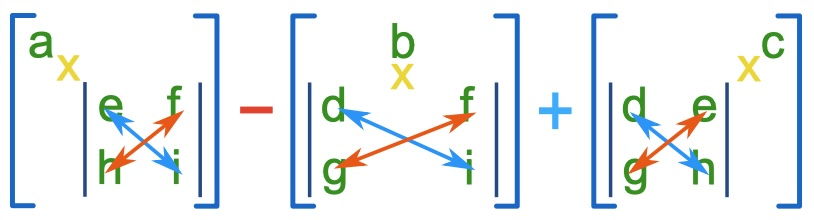
\includegraphics[width=0.5\columnwidth]{images/determinant}}

\begin{align*}
	\det
	\begin{bmatrix}
		a & b \\
		c & d
	\end{bmatrix}
	=
	ad-bc
\end{align*}
\begin{align*}
	\det
	\begin{bmatrix}
		a & b & c \\
		d & e & f \\
		g & h & i
	\end{bmatrix}
	=
	a(ei-fh)-b(di-fg)+c(dh-eg)
\end{align*}

\subsubsection{Properties}
\begin{itemize}
	\item $\det\left(A^{-1}\right) = \frac{1}{\det(A)}$
	\item $\det(A^T) = \det(A)$
	\item $\det(I) = 1$
	\item $\det(cA) = c^n\det(A)\quad(\text{for an }n\times n\text{ matrix})$
	\item $\det(AB) = \det(A)\det(B)$
	\item $\det(A) = \prod_{i=1}^n \lambda_i$
\end{itemize}

\subsection{Particular Solutions to Simple ODEs}

\begin{tabular}[h]{rcl}
    $f'(x)=\frac{c}{x}f(x)$ & $\Rightarrow$ & $f(x)=k_1y^c$                                             \\
    $f'(x)=c\cdot f(x)$     & $\Rightarrow$ & $f(x)=k_1e^{cx}$                                          \\
    $f''(x) = c\cdot f(x)$  & $\Rightarrow$ & $f(x) = k_1e^{\sqrt{c}x}+k_2e^{-\sqrt{c}x}$               \\
    $f''(x) = -c\cdot f(x)$ & $\Rightarrow$ & $f(x)=k_1\sin(\sqrt{c}x)+k_2\cos(\sqrt{c}x)$              \\
    $f'(x)+af(x) = b$       & $\Rightarrow$ & $f(x) = \left(f(0)-\frac{b}{a}\right)e^{-ax}+\frac{b}{a}$
\end{tabular}

\subsection{Harmonic Function}

A function is harmonic if it fulfils $\Delta f = 0$. The mean value property applies:
\begin{align*}
    u(x) = \frac{1}{\mu(S_r(x))}\int_{S_r(x)}u(y)\ d\mu(y)
\end{align*}

\subsection{Polar Coordinates}
\begin{align*}
    x = r\cos \varphi \\
    y = r\sin \varphi \\
\end{align*}
\begin{align*}
    r & = \sqrt{x^2+y^2}\quad{\color{gray} \text{(!) when converting } x^2+y^2\text{, it's }r^2!} \\
    \varphi & = \mathrm{atan2}\left(\frac{y}{x}\right)
\end{align*}

The Laplace operator in polar coordinates is
\begin{align*}
    \Delta u & = \frac{1}{r}\frac{\partial}{\partial r}
    \left(r\frac{\partial u}{\partial r}\right)
    +\frac{1}{r^2}\frac{\partial^2 u}{\partial \varphi^2} \\
    & = \frac{\partial^2 u}{\partial r^2}+\frac{1}{r}\frac{\partial u}{\partial r} +
    \frac{1}{r^2}\frac{\partial^2 u}{\partial \varphi^2}
\end{align*}

\subsection{Tridiagonal Matrix}
\begin{align*}
    M = \mathrm{tridiag}_{n}(a, b, c) =
    \begin{bmatrix}
        b & c &        &        &        &   \\
        a & b & c      &        &        &   \\
        & a & b      & c      &        &   \\
        &   & \ddots & \ddots & \ddots &   \\
        &   &        & a      & b      & c \\
        &   &        &        & a      & b
    \end{bmatrix}_{\color{gray}n\times n}
\end{align*}
